\chapter{Results and Discussion}

\section{Sequences and Static Structures}
\begin{figure}[h!]
	\label{MSA + RMSDs}
	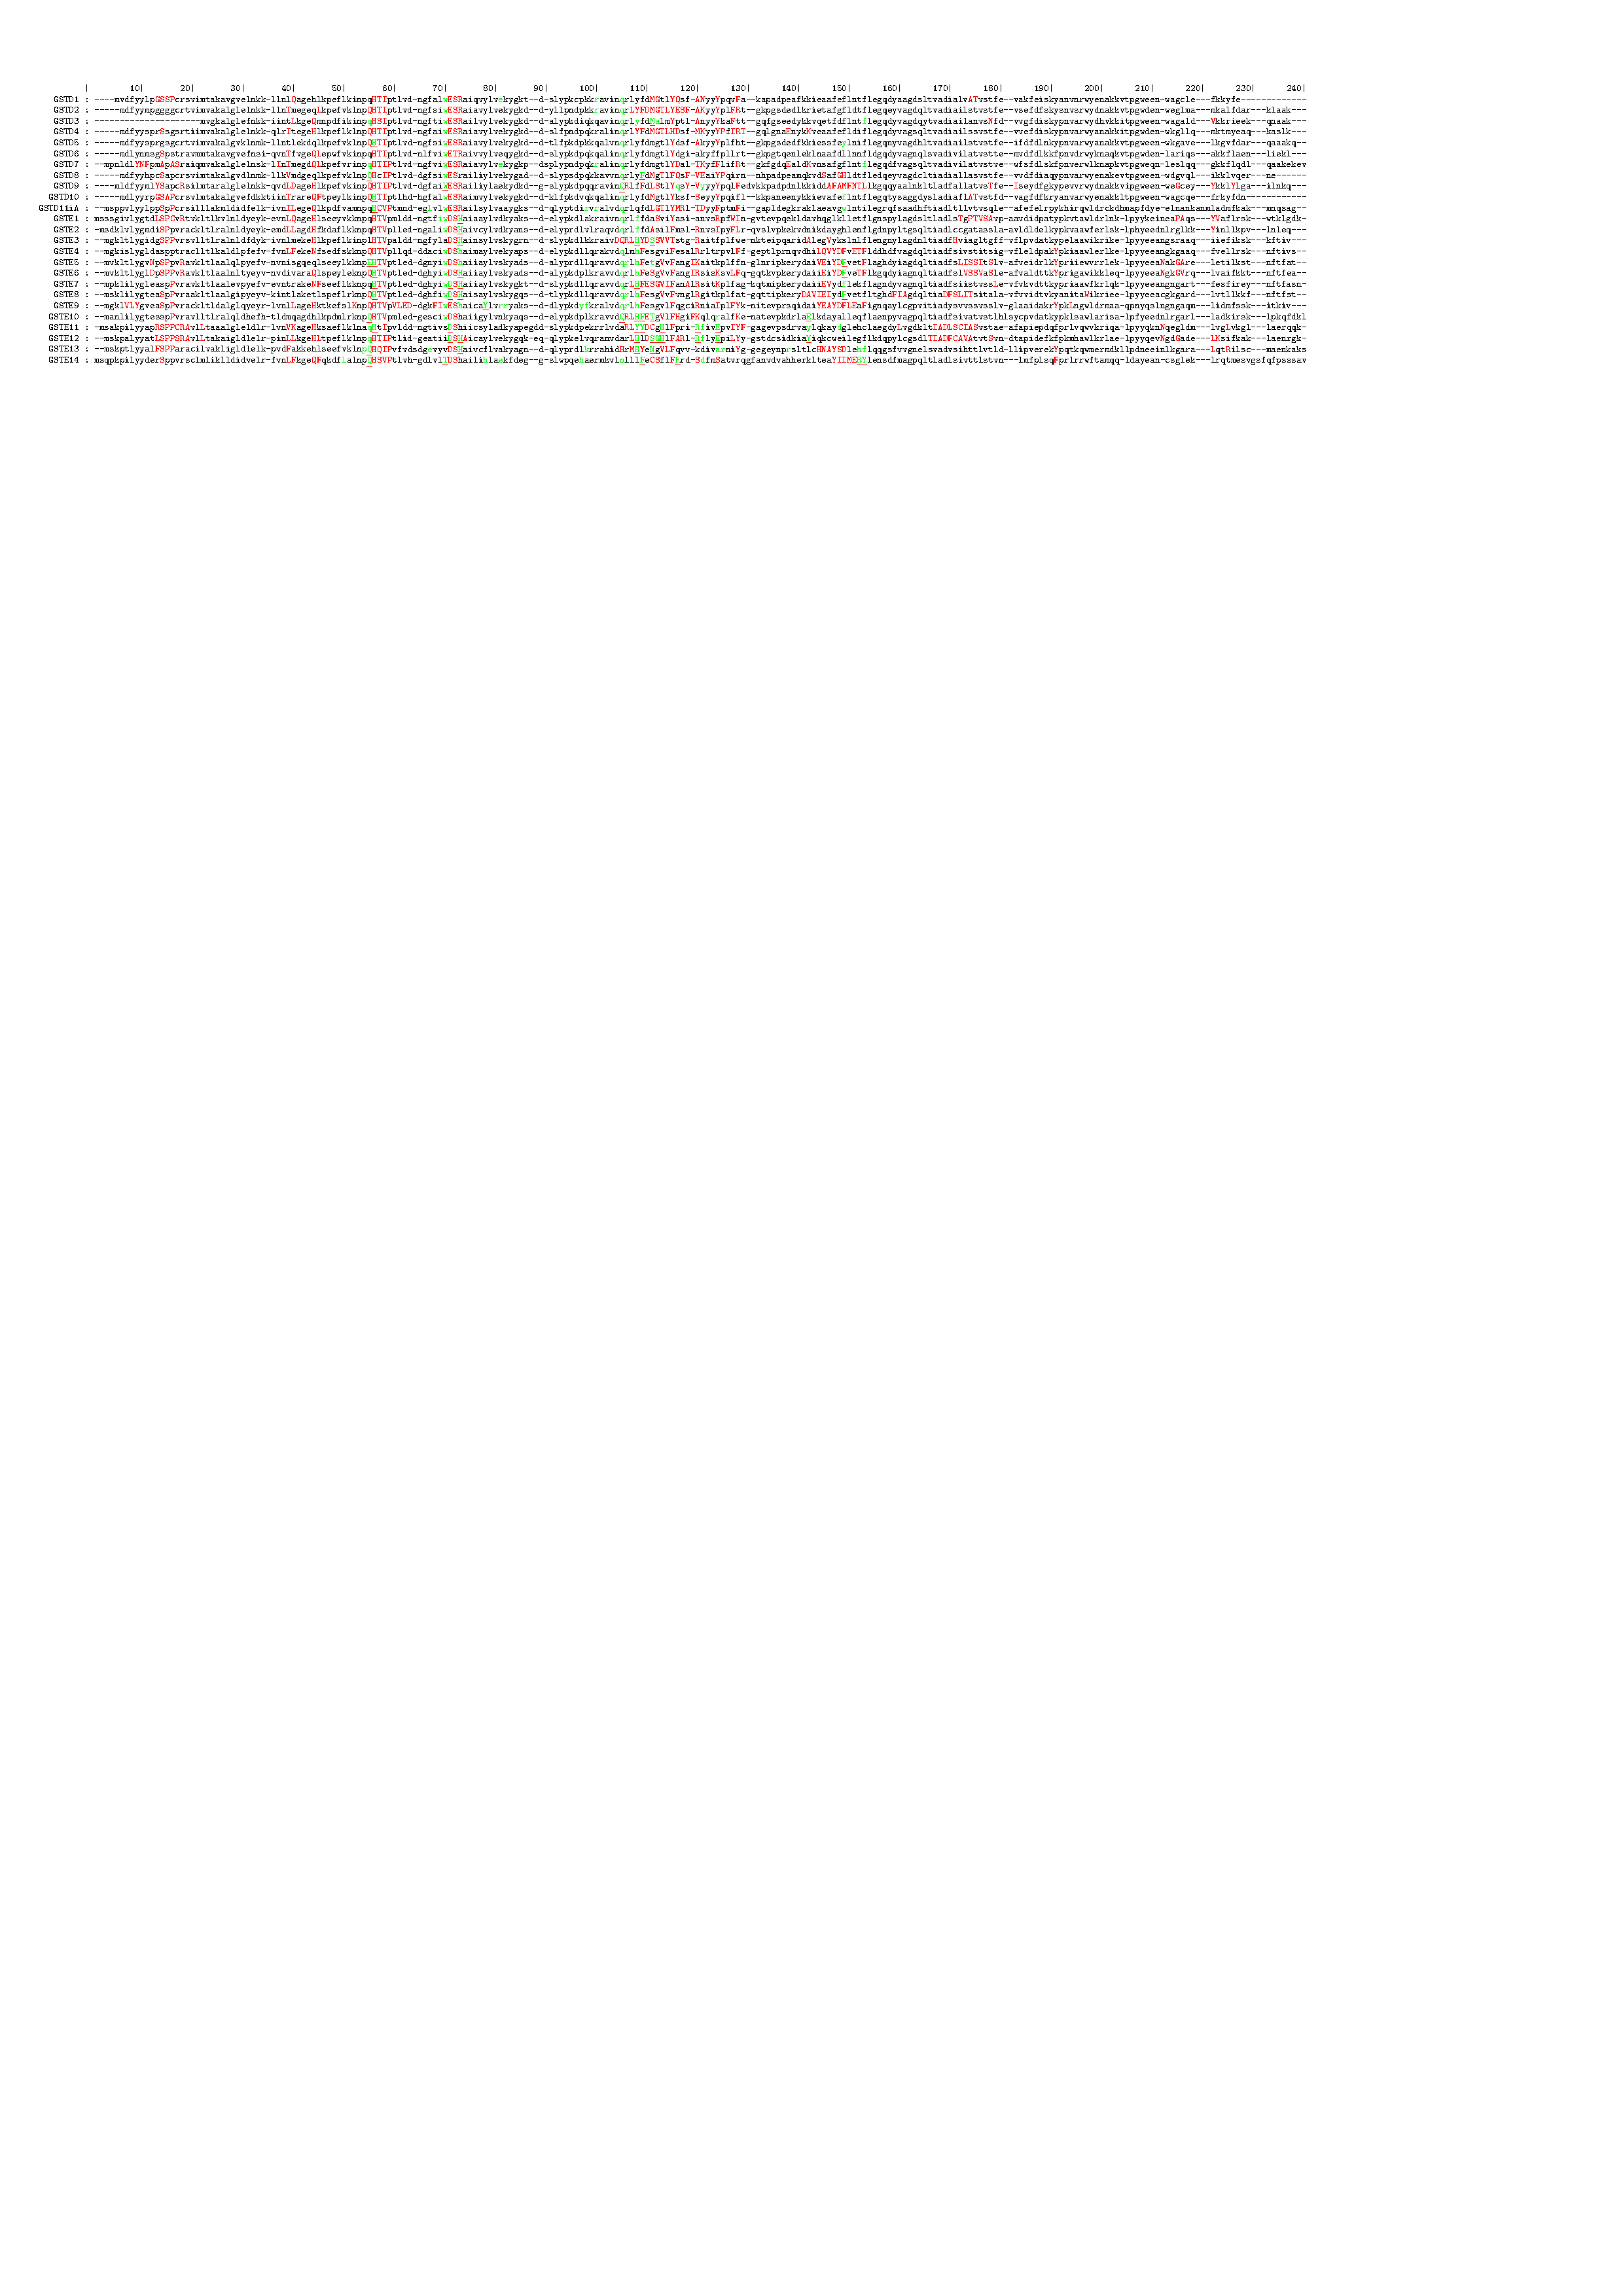
\includegraphics[width = .99\textwidth]{figures/fig3-1-1}\\[.5cm]
	\begin{minipage}{.32\linewidth}
		\includegraphics[width = .99\textwidth]{figures/fig3-1-2}
	\end{minipage}
	\begin{minipage}{.32\linewidth}
		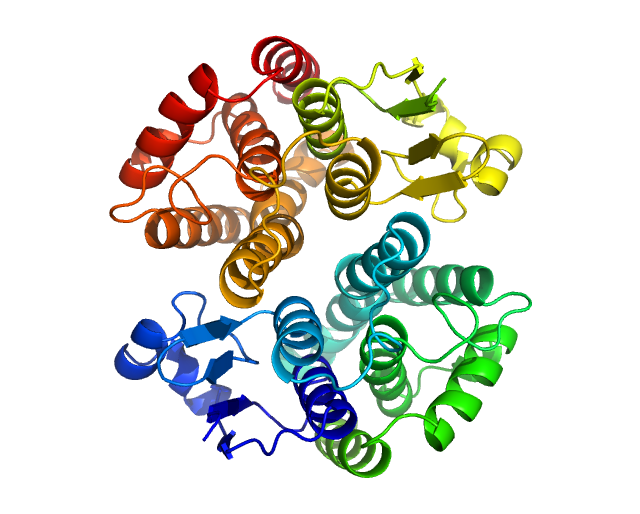
\includegraphics[width = .99\textwidth]{figures/fig3-1-3} % 3ein APO
	\end{minipage}
	\begin{minipage}{.32\linewidth}
		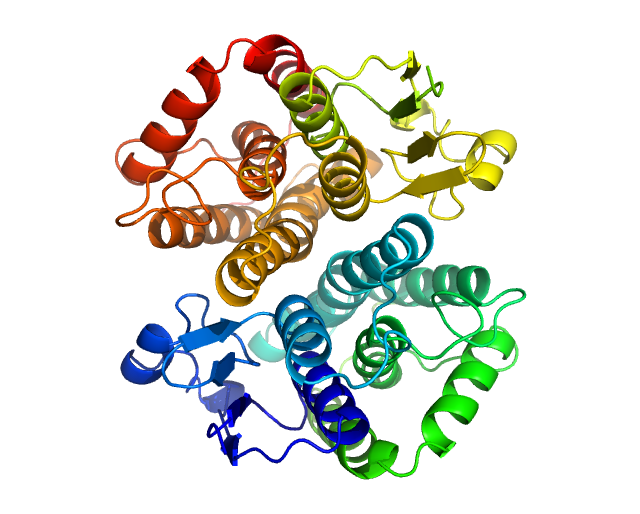
\includegraphics[width = .99\textwidth]{figures/fig3-1-4} % 4png APO
	\end{minipage}
	\caption{MSA \& RMSD matrix of the considered GSTs}
\end{figure}
\noindent As a preliminary analysis, the $25$ sequences of GSTs were aligned using MSA algorithms and structures were predicted using AlphaFold. This allowed us to determine from MSA the conseved regions for the binding site (highlighted in green) and the structural differences between each structure based on the RMSD matrix. In the class $\delta$, the residues in a MSA index of $70-76$ present a very high degree of conservation, and the same goes for the residues $204-210$ in the class $\varepsilon$. Conserved regions are a first probe for the common function of proteins, mainly catalyse in the case of GSTs. Moreover, the programm AlphaFill also allows to predict the position of ligands in the structures and thiuss determine the residues involved in the protein/ligands binding. Here, it clearly appears that the ligands usually binds in the regions $55-58$; $71-73$; $111-121$ with a high conservation but also in region $144-153$ of class $\varepsilon$ with a much smaller conservation. From a geometrical point of view, the structures in class $\delta$ are self similar (with RMSDs between $1$ and $2$ \AA) and structures in class $\varepsilon$ are also self similar but with some exceptions like the GSTE10, GSTE13 and GSTE14 that can either be exceptions from a biological point of view or different because of the precision of the predictions of AlphaFold (with RMSDs $\approx 4$ \AA). Finally, the interface of dimerization looks well conserved from a positional point of view but also from a chemical point of view, with a lot of chemically similar residues in the associated interfaces.   
\section{Dynamics from Normal Modes}

\section{Dynamics from Molecular Dynamics}

\section{Comparison between Structures}